\subsection{IFIT Subcellular Localisation During Interferon Induction and RSV Infection} \label{subsec:IFIT Subcellular Localisation During Interferon INduction and RSV Infection}
put antibody validation wbs

compare and contrast to the info in databases and papers

% introduction to ib stuff from my study
write about ib size statistics from my analysis

\begin{figure}
    \centering
    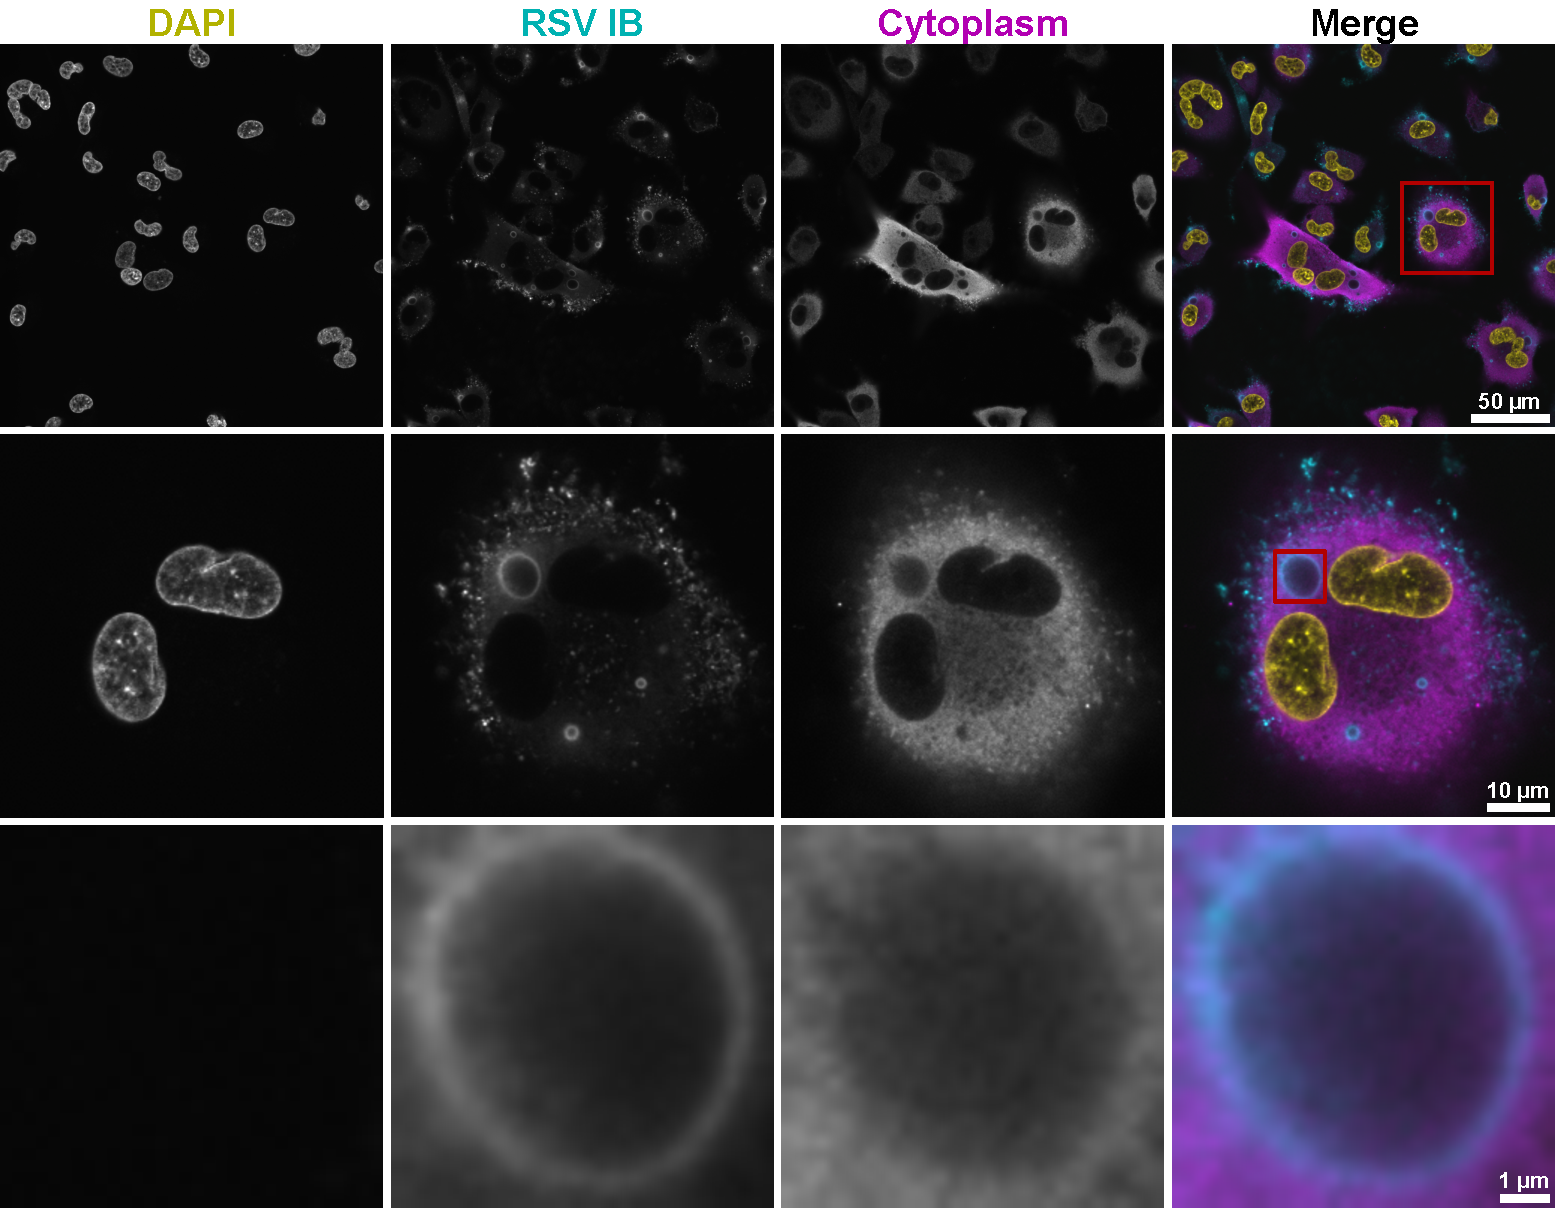
\includegraphics[width=1\linewidth]{09. Chapter 4/Figs/01. Localisation introduction/01. IB-zooms.pdf}
    \caption[Representative Infection Zoom.]{\textbf{Representative Infection Zoom.} asdf asdf asdf asdf asdf asdf sdfgsdfg}
    \label{fig:Representative Infection Zoom}
\end{figure}


\begin{figure}
    \begin{subfigure}{0.5\textwidth}
        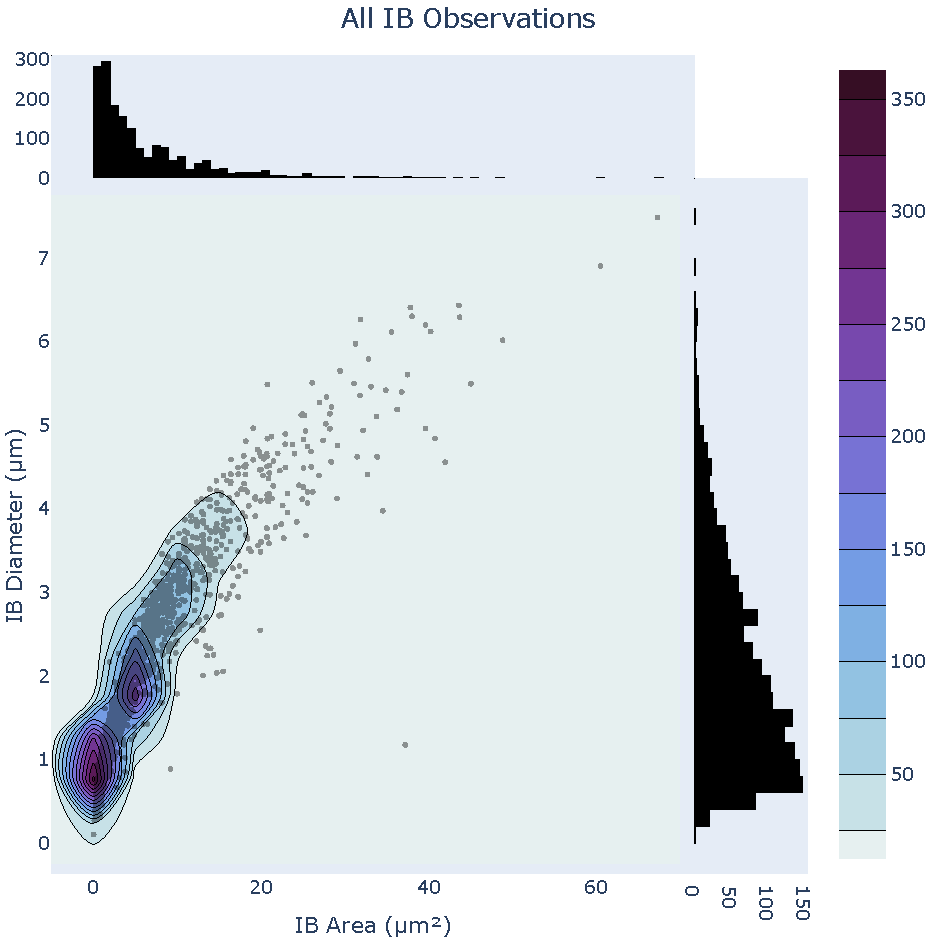
\includegraphics[width=\textwidth]{09. Chapter 4/Figs/01. Localisation introduction/02. heatmap_all.pdf} 
        \caption[]{Size vs Diameter all}
    \end{subfigure}
    \hfill
    \begin{subfigure}{0.5\textwidth}
        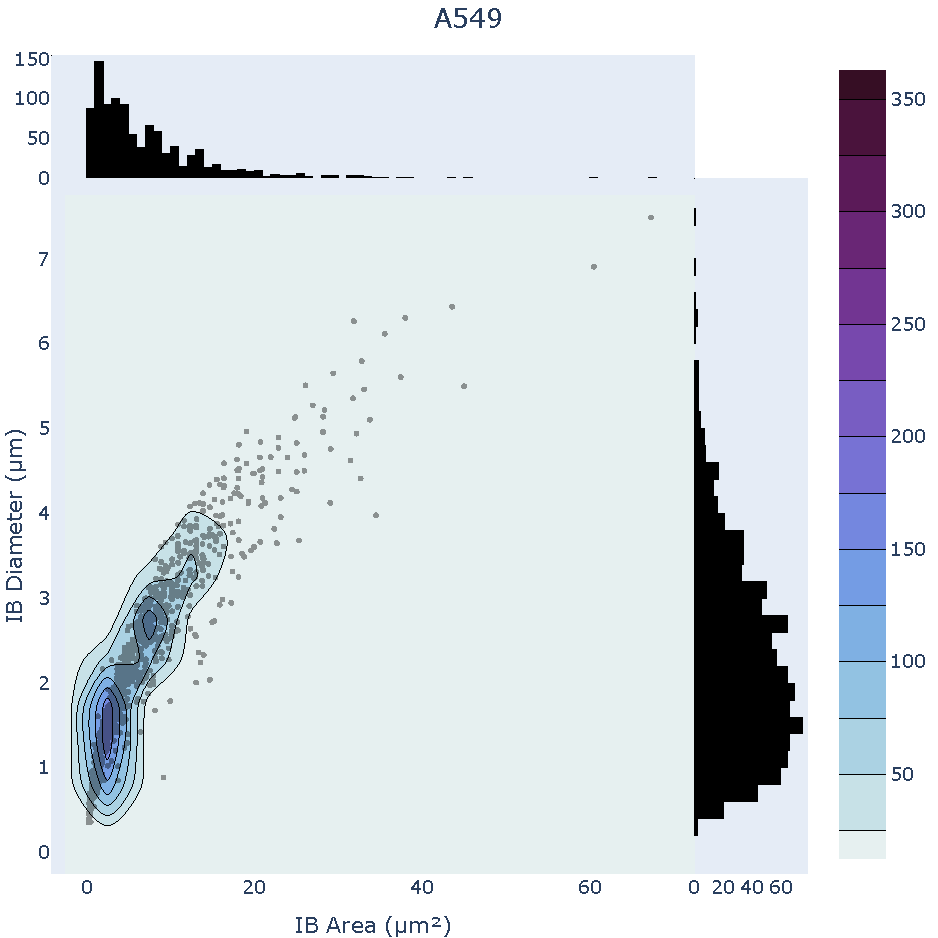
\includegraphics[width=\textwidth]{09. Chapter 4/Figs/01. Localisation introduction/03. heatmap_a549.pdf}
        \caption[]{Size vs Diameter a549}
    \end{subfigure}

    \medskip
    \begin{subfigure}{0.5\textwidth}
        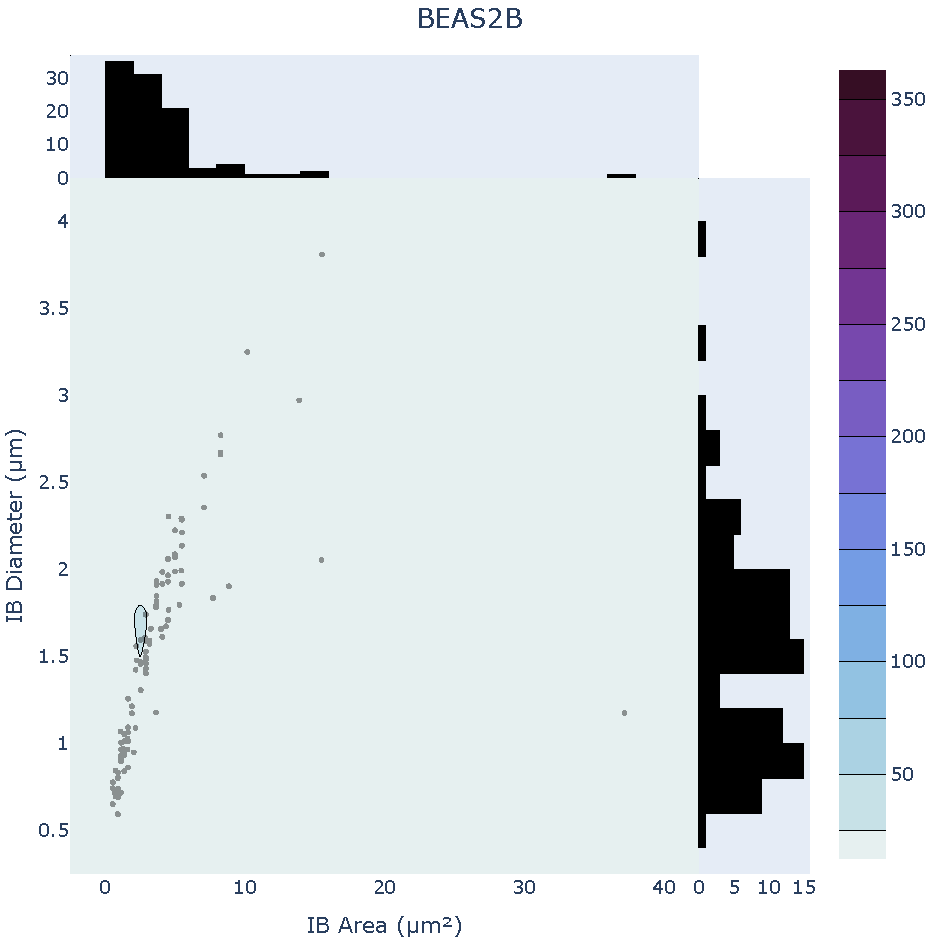
\includegraphics[width=\textwidth]{09. Chapter 4/Figs/01. Localisation introduction/04. heatmap_beas2b.pdf} 
        \caption[]{Size vs Diameter beas2b}
    \end{subfigure}
    \hfill
    \begin{subfigure}{0.5\textwidth}
        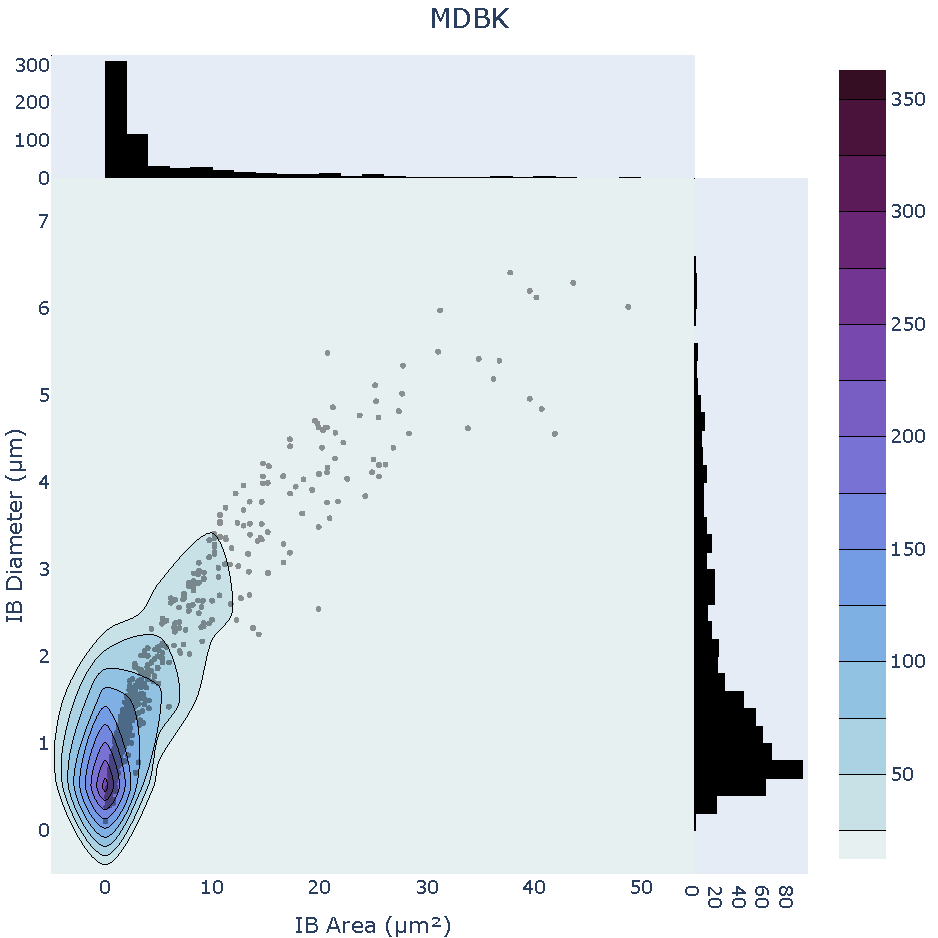
\includegraphics[width=\textwidth]{09. Chapter 4/Figs/01. Localisation introduction/05. heatmap_mdbk.pdf} 
        \caption[]{Size vs Diameter mdbk}
    \end{subfigure}
    
    \caption[size vs diameter of ib all and per cell line]{size vs diameter of ib all and per cell line}
    \label{fig:size vs diameter of ib all and per cell line}
    
\end{figure}


% human stuff
Asdfasfsdfasdf \newline
IF Mock | INF | Infection \newline
A549 BEAS2B

Merge pictures of clusters of cells looking at changes between subcellular localisation and a clear increase in mean intensity. Graphs show mean intensity changes from all cells imaged.

\begin{figure}
    \centering
    \includegraphics[width=1\linewidth]{09. Chapter 4/Figs/01. Localisation introduction/06. a549 merges.pdf}
    \caption[A549 localisation mergers.]{A549 localisation mergers.}
    \label{fig:A549 localisation mergers.}
\end{figure}


\begin{figure}
    \centering
    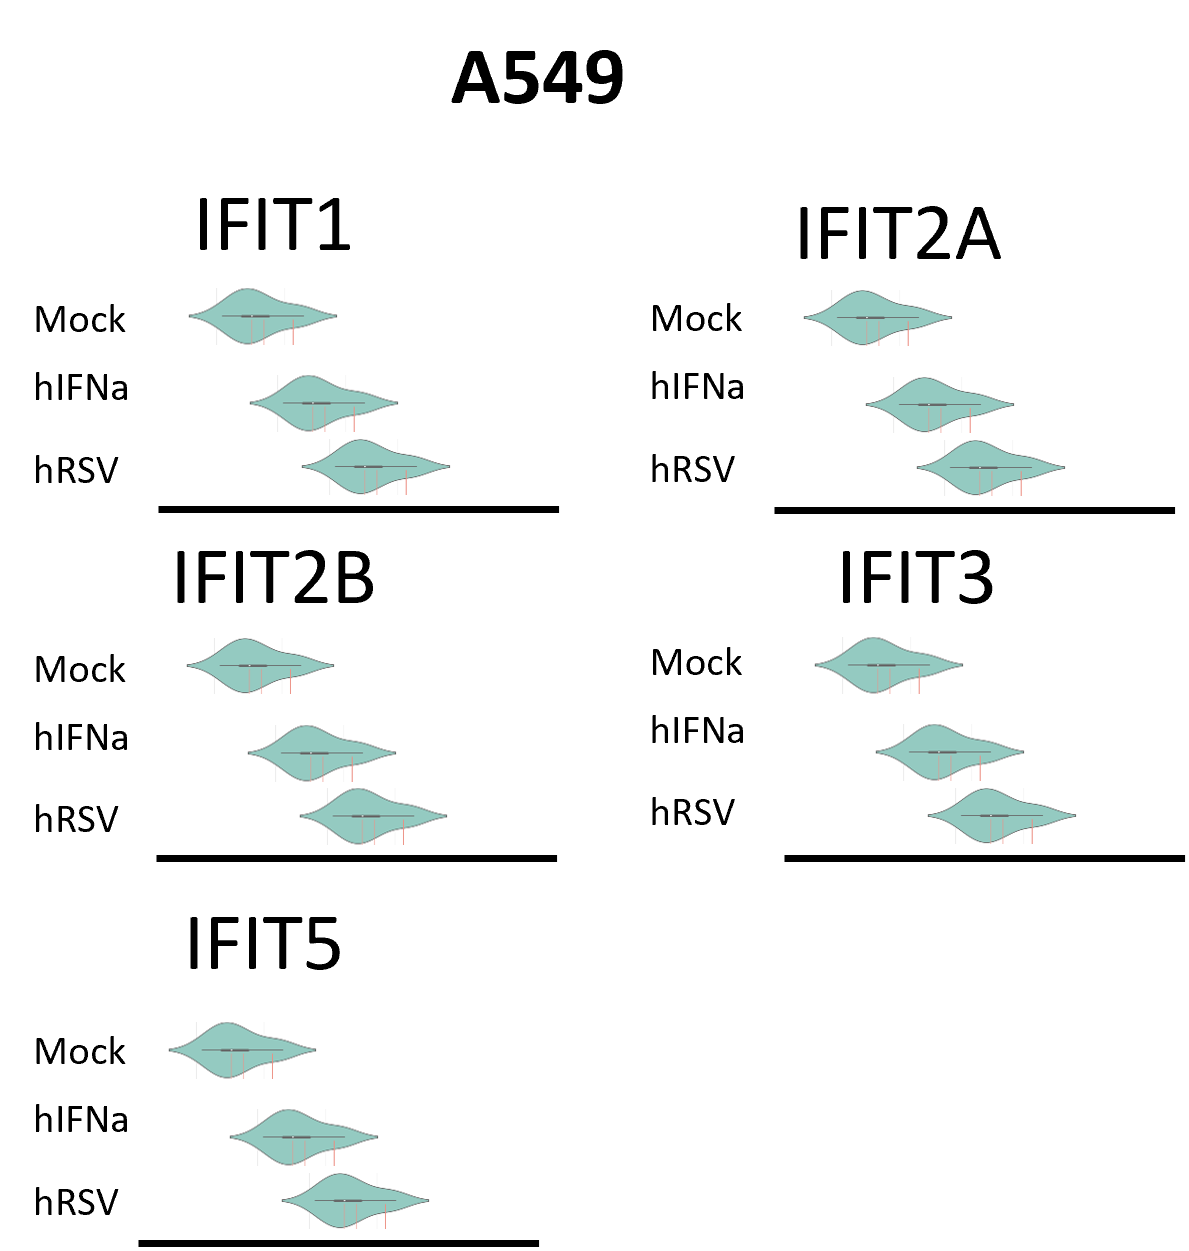
\includegraphics[width=1\linewidth]{09. Chapter 4/Figs/01. Localisation introduction/07. a549 plots.png}
    \caption[A549 localisation plots.]{A549 localisation plots.}
    \label{fig:A549 localisation plots.}
\end{figure}


% bovine stuff
Asdfasfsdfasdf \newline
IF Mock | INF | Infection \newline
MDBK BT

Merge pictures of clusters of cells looking at changes between subcellular localisation and a clear increase in mean intensity. Graphs show mean intensity changes from all cells imaged.

\begin{figure}
    \centering
    \includegraphics[width=1\linewidth]{09. Chapter 4/Figs/01. Localisation introduction/08. mdbk-merges-test.pdf}
    \caption[MDBK localisation mergers.]{MDBK localisation mergers.}
    \label{fig:MDBK localisation mergers}
\end{figure}


\begin{figure}
    \centering
    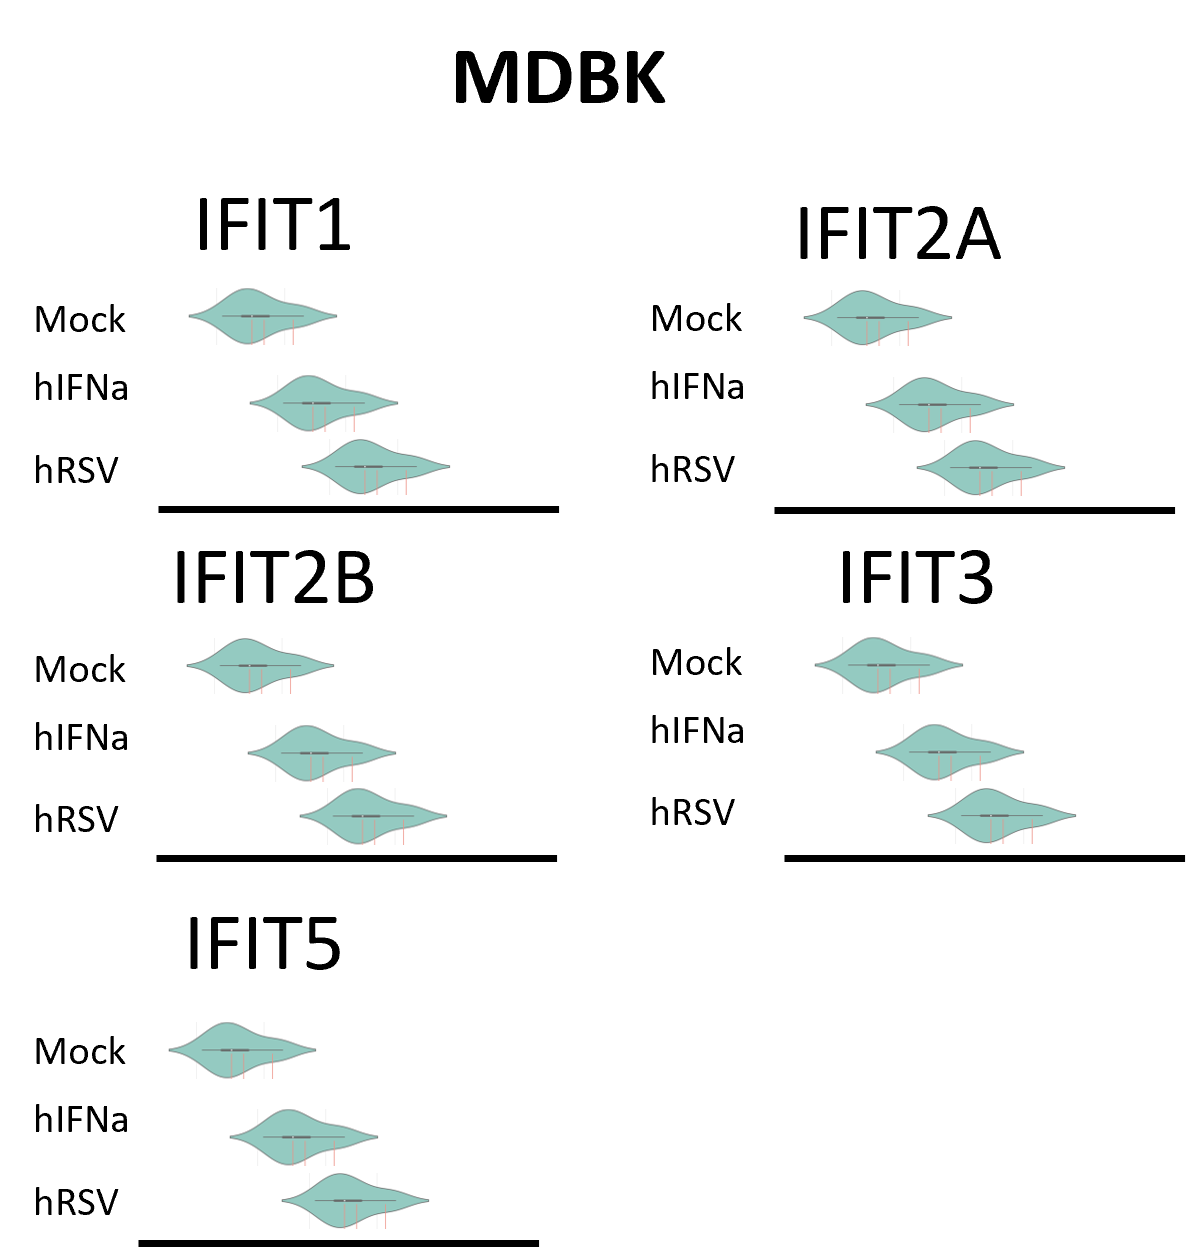
\includegraphics[width=1\linewidth]{09. Chapter 4/Figs/01. Localisation introduction/09. mdbk plots.png}
    \caption[MDBK localisation plots.]{MDBK localisation plots.}
    \label{fig:MDBK localisation plots}
\end{figure}
